% первая часть

\section{Программный язык и среда разработки}

\subsection{Java}

На сегодняшний момент язык Java является одним из самых распространенных и популярных языков программирования. Первая версия языка появилась еще в 1996 году в недрах компании Sun Microsystems, впоследствии поглощенной компанией Oracle. Java задумывался как универсальный язык программирования, который можно применять для различного рода задач. И к настоящему времени язык Java проделал большой путь, было издано множество различных версий. Текущей версией является Java 18, которая вышла 22 марта 2022 года. А Java превратилась из просто универсального языка в целую платформу и экосистему, которая объединяет различные технологии, используемые для целого ряда задач: от создания десктопных приложений до написания крупных веб-порталов и сервисов. Кроме того, язык Java активно применяется для создания программного обеспечения для множества устройств: обычных ПК, планшетов, смартфонов и мобильных телефонов и даже бытовой техники. Достаточно вспомнить популярность мобильной ОС Android, большинство программ для которой пишутся именно на Java.

\subsubsection{Язык Java}

Ключевой особенностью языка Java является то, что его код сначала транслируется в специальный байт-код, независимый от платформы. А затем этот байт-код выполняется виртуальной машиной JVM (Java Virtual Machine). В этом плане Java отличается от стандартных интерпретируемых языков как PHP или Perl, код которых сразу же выполняется интерпретатором. В то же время Java не является и чисто компилируемым языком, как С или С++.

Подобная архитектура обеспечивает кроссплатформенность и аппаратную переносимость программ на Java, благодаря чему подобные программы без перекомпиляции могут выполняться на различных платформах - Windows, Linux, Mac OS и т.д. Для каждой из платформ может быть своя реализация виртуальной машины JVM, но каждая из них может выполнять один и тот же код.

Java является языком с Си-подобным синтаксисом и близок в этом отношении к C/C++ и C\#. Поэтому, если вы знакомы с одним из этих языков, то овладеть Java будет легче.

Еще одной ключевой особенностью Java является то, что она поддерживает автоматическую сборку мусора. А это значит, что вам не надо освобождать вручную память от ранее использовавшихся объектов, как в С++, так как сборщик мусора это сделает автоматически за вас.

Java является объектно-ориентированным языком. Он поддерживает полиморфизм, наследование, статическую типизацию. Объектно-ориентированный подход позволяет решить задачи по построению крупных, но в тоже время гибких, масштабируемых и расширяемых приложений.

По данным компании Oracle, программы на Java запускаются на 3 млрд девайсов. Это маркетинговое сообщение сложно проверить. Тем не менее Java широко используется и входит в число самых востребованных языков, это не вызывает сомнения.

Например, подавляющее большинство крупных компаний так или иначе используют Java. Очень много серверных приложений для корпораций написаны на этом языке. Например, речь идёт о программах для финансовых организаций, которые обеспечивают проведение транзакций, фиксацию торговых операций.

На Java написано много веб-приложений. Популярные фреймворки, в том числе Spring, Stuts, JSP, используются для создания разных приложений в вебе: от ecommerce-проектов до крупных порталов, от образовательных платформ до правительственных ресурсов.

Мобильная разработка — ещё одна область использования Java. На этом языке пишут приложения для устройств, работающих под управлением ОС Android.

На Java создают клиентские приложения. Простой и близкий разработчикам пример: IDE NetBeans написано на «джаве».

Также Java применяется для работы с Big Data, разработки программ для научных целей, например, обработки естественных языков, программирования приборов — от бытовых девайсов до промышленных установок.

То есть на Java можно писать разные типы приложений: веб, мобильный и десктопный софт, игры и так далее. Традиционно у этого языка сильные позиции в промышленном программировании, в сегменте крупных компаний (т.н. энтерпрайз).

Java — достаточно распространённый язык: им пользуется большое количество разработчиков, и решение практически любой проблемы, которая может возникнуть при работе с Java, уже кто-то придумал. Благодаря тысячам библиотек и форумов, можно найти готовое решение почти в любой ситуации. На GitHub, например, есть открытые проекты и документация, а на форуме Stack Overflow можно обратиться за помощью к комьюнити.

Язык Java строго типизирован. То есть любая переменная или выражение имеет определённый тип уже на момент компиляции, что упрощает выявление каких-либо проблем. Компилятор сам подсказывает программисту, где тот допускает ошибку, и не даёт её совершить.

Все библиотеки, написанные когда-либо для Java, — это классы, которые отвечают за функциональность языка. Любое приложение на Java — набор классов, описывающих разные объекты. Это хорошо, потому что позволяет создавать сложные программы, но простые в поддержке. И в целом Java — мультипарадигменный язык, то есть поддерживает множество принципов программирования, что позволяет эффективно решать разные задачи.


\subsubsection{Графический интерфейс в Java}

GUI (графический интерфейс пользователя) в Java — это простой в использовании конструктор визуального восприятия для Java-приложений. Он состоит в основном из графических компонентов, таких как кнопки, ярлыки, окна и т.д., с помощью которых пользователь может взаимодействовать с приложением. GUI играет важную роль в создании простых интерфейсов для Java-приложений.

Графический интерфейс в Java прошел весьма тернистый путь развития и становления. Долгое время его обвиняли в медленной работе, жадности к ресурсам системы и ограниченной функциональности.

Первой попыткой Sun создать графический интерфейс для Java была библиотека AWT (Abstract Window Toolkit) — инструментарий для работы с различными оконными средами. Sun сделал прослойку на Java, которая вызывает методы из библиотек, написанных на С. Библиотечные методы AWT создают и используют графические компоненты операционной среды. С одной стороны, это хорошо, так как программа на Java похожа на остальные программы в рамках одной ОС. Но при запуске ее на другой платформе могут возникнуть различия в размерах компонентов и шрифтов, которые будут портить внешний вид программы.

Чтобы обеспечить мультиплатформенность AWT интерфейсы вызовов компонентов были унифицированы, вследствие чего их функциональность получилась немного урезанной. Да и набор компонентов получился довольно небольшой. Так, например, в AWT нет таблиц, а в кнопках не поддерживается отображение иконок. Тем не менее, пакет java.awt входит в Java с самого первого выпуска и его можно использовать для создания графических интерфейсов.

Таким образом, компоненты AWT не выполняют никакой "работы". Это просто «Java-оболочка» для элементов управления той операционной системы, на которой они работают. Все запросы к этим компонентам перенаправляются к операционной системе, которая и выполняет всю работу.

Использованные ресурсы AWT старается освобождать автоматически. Это немного усложняет архитектуру и влияет на производительность. Написать что-то серьезное с использованием AWT будет несколько затруднительно. Сейчас ее используют разве что для апплетов.

Вслед за AWT Sun разработала графическую библиотеку компонентов Swing, полностью написанную на Java. Для отрисовки используется 2D, что принесло с собой сразу несколько преимуществ. Набор стандартных компонентов значительно превосходит AWT по разнообразию и функциональности. Swing позволяет легко создавать новые компоненты, наследуясь от существующих, и поддерживает различные стили и скины.

Создатели новой библиотеки пользовательского интерфейса Swing не стали «изобретать велосипед» и в качестве основы для своей библиотеки выбрали AWT. Конечно, речь не шла об использовании конкретных тяжеловесных компонентов AWT (представленных классами Button, Label и им подобными). Нужную степень гибкости и управляемости обеспечивали только легковесные компоненты. На диаграмме наследования (рисунок~\ref{fig:swing-base}) представлена связь между AWT и Swing.

\begin{figure}[H]
	\centering
	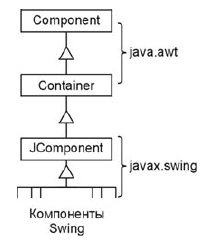
\includegraphics[width=0.5\linewidth]{pics/swing-base}
	\caption{Диаграмма наследования}
	\label{fig:swing-base}
\end{figure}



Важнейшим отличием Swing от AWT является то, что компоненты Swing вообще не связаны с операционной системой и поэтому гораздо более стабильны и быстры. Такие компоненты в Java называются легковесными (lightweight), и понимание основных принципов их работы во многом объяснит работу Swing.

Чтобы понять разницу между AWT и Swing, надо посмотреть на рисунок~\ref{fig:AWT-Swing-diff}.


\begin{figure}[H]
	\centering
	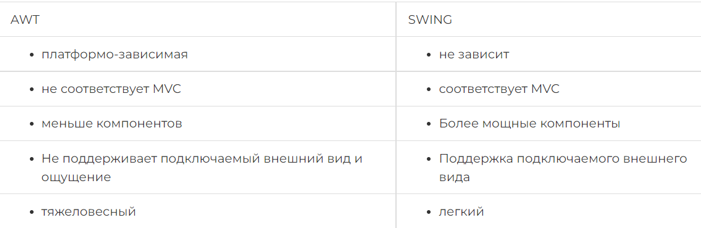
\includegraphics[width=1\linewidth]{pics/AWT-Swing-diff}
	\caption{AWT и Swing}
	\label{fig:AWT-Swing-diff}
\end{figure}

Компонент Swing следует архитектуре Model-View-Controller для выполнения следующих критериев:
\begin{itemize}
\item Одного API должно быть достаточно для поддержки множественного внешнего вида;
\item API должен быть ориентирован на модель, чтобы не требовалось, чтобы у API самого высокого уровня были данные;
\item API заключается в использовании модели Java Bean, чтобы инструменты Builder и IDE могли предоставлять разработчикам более качественные сервисы для использования.
\end{itemize}

Иерархия классов в Swing представлена на рисунке~\ref{fig:hierarchy}.
\begin{figure}[H]
	\centering
	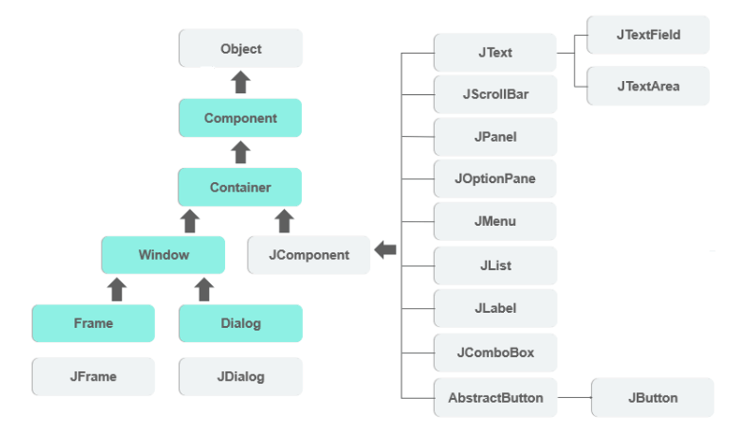
\includegraphics[width=1\linewidth]{pics/hierarchy}
	\caption{Иерархия классов Swing}
	\label{fig:hierarchy}
\end{figure}


Все компоненты в свинге, такие как JButton, JComboBox, JList, JLabel, унаследованы от класса JComponent, который можно добавить в классы контейнера.

Контейнеры – это окна, такие как рамка и диалоговые окна. Основные компоненты являются строительными блоками любого графического приложения. Такие методы, как setLayout, переопределяют макет по умолчанию в каждом контейнере. Контейнеры, такие как JFrame и JDialog, могут добавлять только компонент к себе.

\subsection{Среда разработки NetBeans}

NetBeans IDE - бесплатная интегрированная среда разработки с открытым исходным кодом для разработчиков программного обеспечения. Среда предоставляет все средства, необходимые для создания профессиональных десктоп приложений, корпоративных, мобильных и веб-приложений на платформе Java, а также C/C++, PHP, JavaScript, Groovy и Ruby. 
Основные характеристики NetBeans IDE:


\begin{itemize}
\item рабочая область среды IDE является полностью настраиваемой - существует возможность пользовательской настройки действий, выполняемых с помощью панели, назначения "горячих" клавиш и т.д.;
\item IDE имеет в своем составе расширенный многоязыковой редактор для различных языков программирования - Java, C/C++, Ruby, Groovy, PHP, JavaScript, CSS, XML, HTML, RHTML, JSP, документацию Javadoc. Существует возможность расширения функций редактора с целью поддержки любого другого языка;
\item производится проверка ошибок во время ввода, отображение вариантов для автозавершения кода и фрагментов документации по требуемому языку программирования;
\item редактор может генерировать и вставлять в исходный код стандартные фрагменты кода на Java или других языках;
\item браузер классов позволяет просматривать иерархию и структуру любого класса Java - отображаются интерфейсы, базовые классы, производные классы и члены классов;
\item существует возможность перемещения любой вкладки редактора в пределах рабочего пространства IDE и за её пределы, создавая независимое окно, которое можно переместить на второй экран;
\item возможность группирования связанных проектов - создавая группы проектов, можно быстро открывать и закрывать несколько сгруппированных проектов одновременно;
\item расширенные средства для выполнения контекстно-зависимого поиска по всей среде IDE, справочным материалам и всем открытым проектам и файлам;
\item существует возможность создания проектов в свободном формате или начинать работу с проектом с шаблона. В комплекте со средой IDE поставляются шаблоны и примеры проектов для приложений Java SE, мобильных, веб-приложений и приложений уровня предприятия, приложений JavaFX, подключаемых модулей NetBeans, приложений Groovy, PHP, C/C++, Ruby и Ruby on Rails;
\item NetBeans IDE является платформой для построения десктоп приложений с функциональным пользовательским интерфейсом, т.к. представляет из себя фреймворк к Java библиотеке Swing;
\item NetBeans имеет встроенную поддержку CVS, Mercurial и Subversion. Для просмотра изменений используется редактор с цветовыми обозначениями.
\end{itemize}

Возможности программирования в NetBeans:
\begin{itemize}
\item разработка Java десктоп приложений с профессиональными графическими интерфейсами пользователя. Используется визуальный редактор - Swing GUI Builder. Работа осуществляется путем перетаскивания элементов графического интерфейса из палитры на холст. Предварительное позиционирование элементов можно осуществлять с помощью указателя мыши. Панель свойств и инспектор компонентов предоставляют возможность тонкой настройки каждого компонента интерфейса; 
\item создание веб-приложений и корпоративных приложений в соответствии со стандартами. Среда NetBeans предоставляет полную поддержку Java EE 6. Позволяет разрабатывать веб-страницы, сервлеты, веб-сервисы, Enterprise Java Beans (EJB), проекты Java EE с использованием JavaServer Faces 2.0 (Facelets), Spring, Struts и Hibernate;
\item программирование на PHP, поддержка всех сопутствующих языков программирования, технологий и веб-стандартов. Возможность создавать проекты PHP на основе платформы Zend или Symfony. Редактор PHP динамически интегрирован с функциями редактирования HTML, JavaScript и CSS. Проекты PHP могут быть развёрнуты из среды NetBeans на локальном или удаленном сервере при взаимодействии через FTP или SFTP;
\item возможность создания, тестирования, отладки и внедрения приложений, функционирующих на мобильных телефонах, карманных компьютерах, телеприставках и встраиваемых системах. Visual Mobile Designer (VMD) создает всю необходимую модульную инфраструктуру проекта и обеспечивает быструю разработку графических интерфейсов путём перетаскивания в рабочую область компонентов - экран ожидания, экран входа в систему, обозреватель файлов, средство составления сообщений SMS и экран заставки. Возможность создания пользовательского интерфейса на основе SVG;
\item использование JavaFX Composer для визуального структурирования приложения JavaFX с графическим интерфейсом, аналогично конструктору GUI Swing для Java десктоп приложений;
\item возможность разработки профессиональных приложений на языках C, C++ для различных платформ - Windows, Linux, Mac и Solaris. Поддерживаются все широко используемые компиляторы - GNU, Cygwin и MinGW. Существует возможность установки требуемого компилятора, определений препроцессора, параметров времени компиляции и т.д.;
\item расширенные возможности по работе с базами данных - встроенный клиент к базам данных - MySQL, Postgres, Oracle и др., редактор запросов SQL, возможность редактировать таблицы баз данных напрямую через редактор таблиц;
\item интеграция с серверами приложений и контейнерами сервлетов - автоматическое развёртывание приложений, управление сервером - запуск, остановка, перезапуск;
\item многоязычный пользовательский интерфейс с поддержкой русского языка;
\item расширение функциональности с помощью подключаемых модулей, гибкая система управления компонентами, модулями, обновление и загрузка модулей через интернет.

\end{itemize}

NetBeans - единственная IDE, которая устроит и начинающего разработчика и профессионала. Наличие подробной встроенной справочной системы обеспечит быстрый старт для начинающих пользователей.

